\documentclass[12pt]{article}
\usepackage[utf8]{inputenc}
\usepackage{graphicx}
\usepackage[a4paper, total={6in, 8in}]{geometry}
\usepackage{listings}
\usepackage{color}
\graphicspath{ {images/} }
\usepackage{float}
 
\title{Lab work report 9 - Norm}
\author{Cao Anh Quan - ICT Master}
\date{November 13, 2016}
 
 
\begin{document}
 
\begin{titlepage}
\maketitle
\end{titlepage}

The employee database satisfy the 3NF because:

\begin{enumerate}


\item Determine \emph{Concepts}

\begin{itemize}

\item Magazine
\item Article
\item Author
\begin{figure}[H]
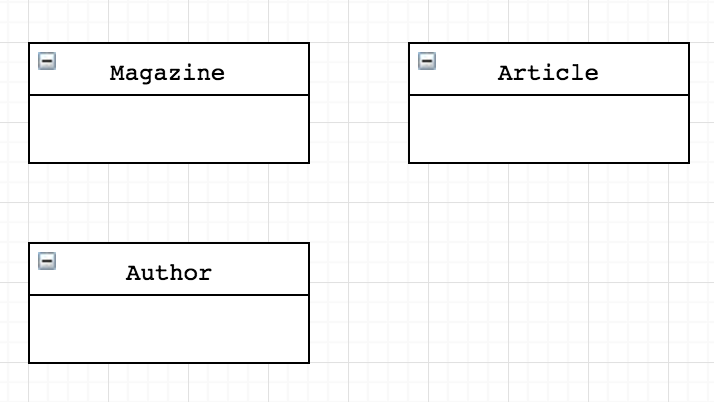
\includegraphics[width=\textwidth]{concept.png}
\end{figure}
\end{itemize}

\item Determine Attributes of each concept
\begin{figure}[H]
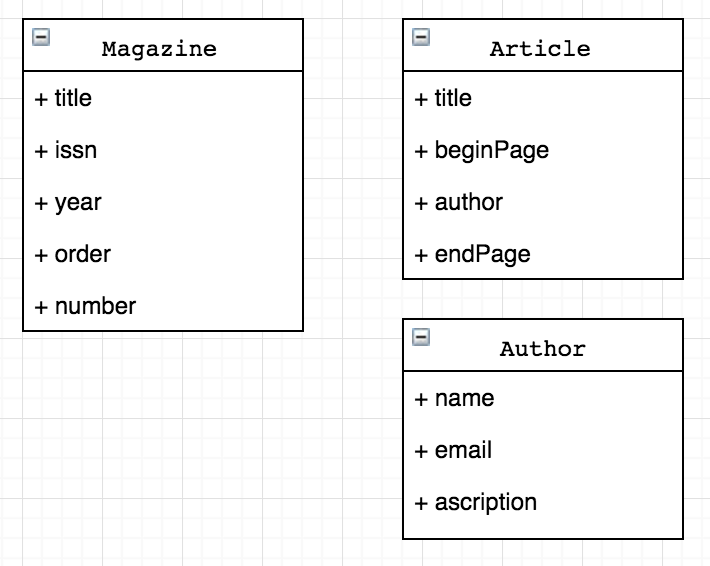
\includegraphics[width=\textwidth]{attributes.png}
\end{figure}


\item Determine links (relationships) between them
\begin{figure}[H]
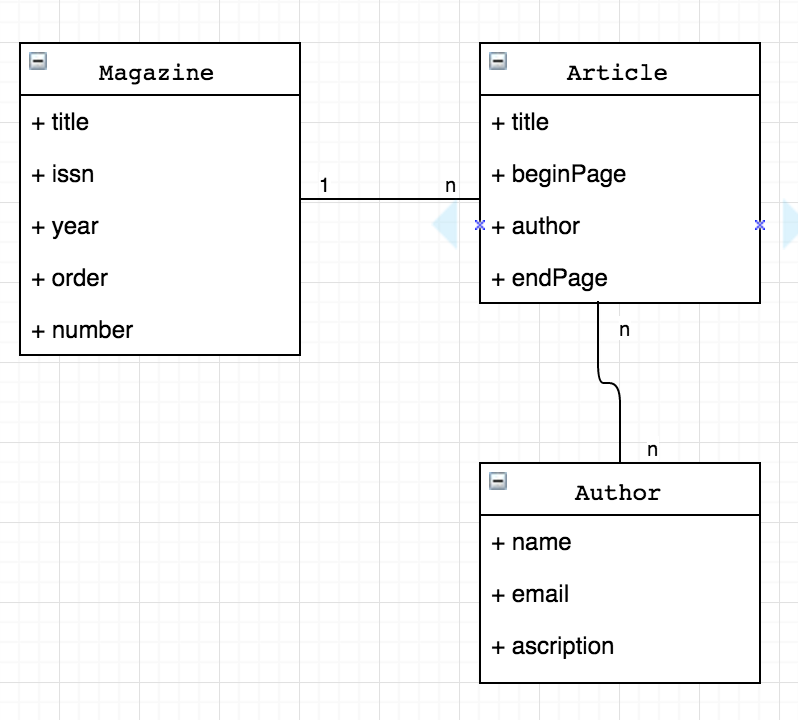
\includegraphics[width=\textwidth]{relations.png}
\end{figure}


\item Determine types of each concept attribute 

\begin{figure}[H]
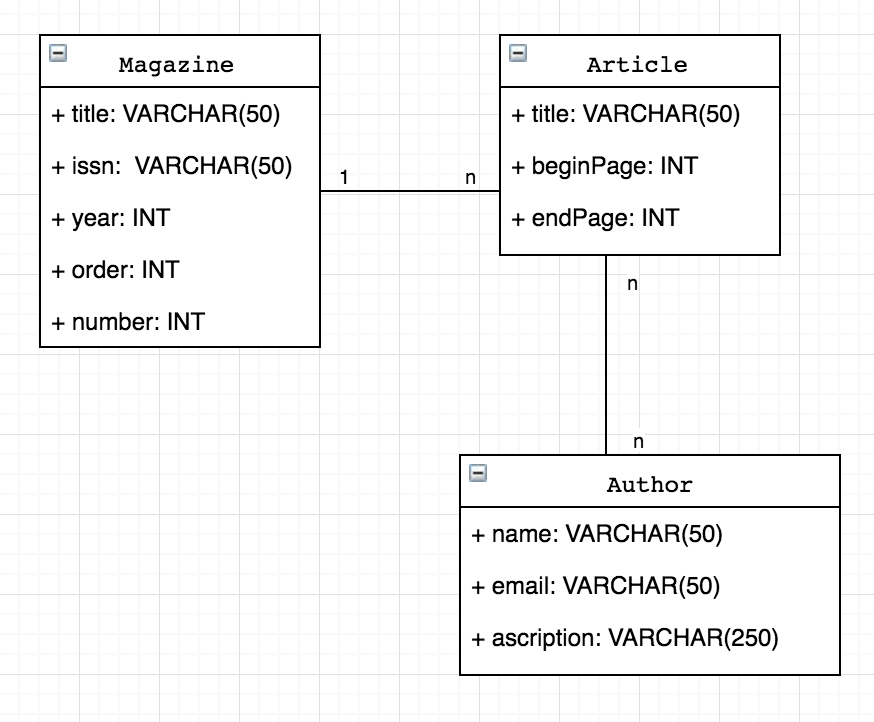
\includegraphics[width=\textwidth]{types.png}
\end{figure}


\item Solve foreign key links

\begin{figure}[H]
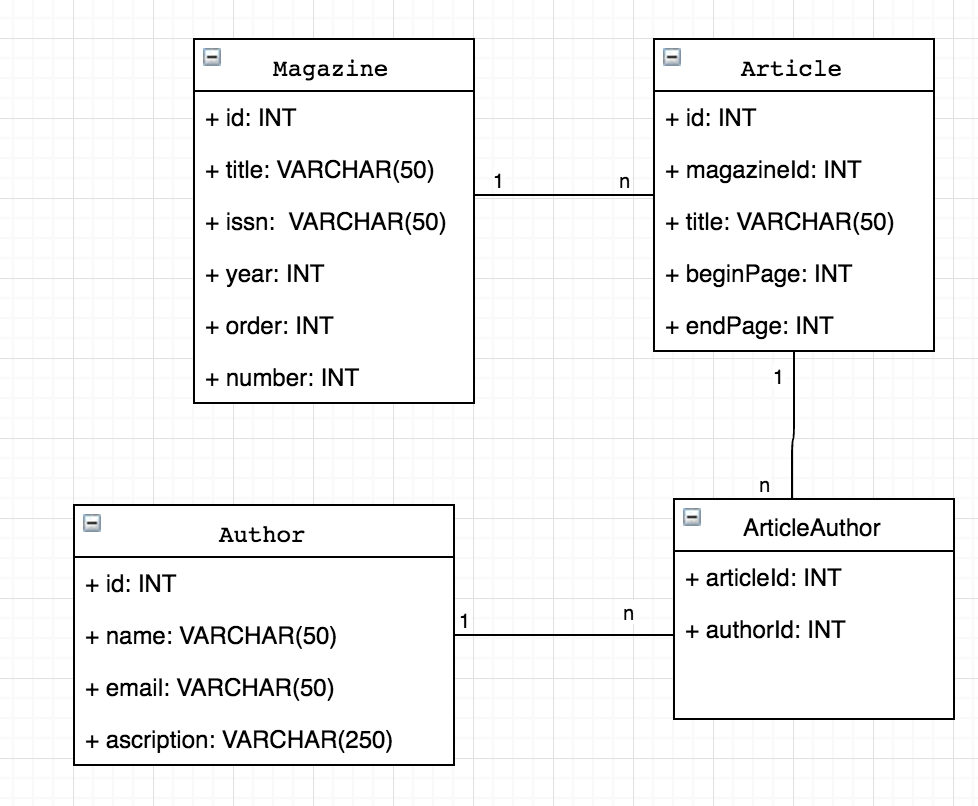
\includegraphics[width=\textwidth]{keys.png}
\end{figure}

\item Implementation

\begin{lstlisting}[language=SQL]

create database magazine;
use magazine;

CREATE TABLE Magazine (
	id INT NOT NULL AUTO_INCREMENT,
	title VARCHAR(50),
	issn VARCHAR(50),
	`year` INT,
	`order` INT,
	number INT,
	PRIMARY KEY (id)
);

CREATE TABLE Article (
	id INT NOT NULL AUTO_INCREMENT,
	magazineId INT NOT NULL,
	title VARCHAR(50),
	beginPage INT,
	endPage INT,
	PRIMARY KEY (id),
	FOREIGN KEY (magazineId) REFERENCES Magazine(id)
);

CREATE TABLE Author (
	id INT NOT NULL AUTO_INCREMENT,
	name VARCHAR(50),
	email VARCHAR(50),
	ascription VARCHAR(250),
	PRIMARY KEY (id)
);


CREATE TABLE ArticleAuthor (
	articleId INT NOT NULL,
	authorId INT NOT NULL,
	PRIMARY KEY (authorId,articleId),
	FOREIGN KEY (articleId) REFERENCES Article(id),
	FOREIGN KEY (authorId) REFERENCES Author(id)
);



\end{lstlisting}



\end{enumerate}




 
\end{document}
